\chapter{Background}

\section{Zebrafish spinal cord regeneration}

%  [describe the process and how cells and cytokines are involved]

Compared to mammals, zebrafish can regenerate spinal cord after injury, and possibly recover swimming function. They are widely used in regenerative ability researches due to this ability. Experiments found that although being cut off, the axonal of nerve cells can regenerate and bridge across the lesion site, which critically determined whether zebrafish can regain the swimming function \cite{axonal}. Tsarouchas et al. \cite{ref:Tsarouchas} studied the the complex interactions happen at the lesion site. The inflammation affects the regeneration, as if it is promoted, it accelerates the axonal regeneration; if it is inhibited, it reduces the regeneration. Further experiments showed that two kinds of cytokines, il-1$\beta$ and tnf-$\alpha$, are related the inflammation, and they are dynamically controlled by immunes cells, i.e. cytokines works as media to control the axonal regeneration. Cytokines are small proteins, work as messenger to pass signal across different cells, which are similar to hormones and neurotransmitter.

An interaction map can be drawn, according to the evidences found by Tsarouchas et al. \cite{ref:Tsarouchas}. After injury, a massive immune response was observed, with the increasing numbers of several kinds of cells: macrophage, neutrophil. This dynamical system consists of complex interactions between cells and cytokines, For example, il-1$\beta$ promotes macrophages' increase, and as a major source, more macrophages leads to more expression of tnf-$\alpha$ mRNA. Consequently as media, tnf-$\alpha$ and il-1$\beta$ plays determinative roles in the axonal regeneration, where generally il-1$\beta$ promotes the regeneration at early stages, but later has an inhibition effect; tnf-$\alpha$ promotes the regeneration all the time. The presence of the cytokines also affects the number of immune cells, while as sources, more cells lead to more expression of cytokines. Interactions between different kinds of cells are also considered in the system.

This dynamic system is suitable for mathematical modelling, where a set of equations can be written to represent the dynamics of different objects e.g. cells and cytokines. Our interest lies in the modelling of the regeneration period of the dynamic system, and we wish to find that if we can quantitatively study the interactions iniside the system, based on the proposed hypothesis \cite{ref:Tsarouchas}, and furthermore based our own hypothesis which may include different interactions.

The biological background of works in this dissertation is mostly related the the experimental evidences, quantitative data and proposed hypothesis in \cite{ref:Tsarouchas}. The published data on the quantitative measurement of cells and cytokines make the modelling and further analysis possible. Some other interactions proposed in our modelling stages are enlightened from Anderson et al. \cite{Anderson}.

\section{Mathematical modelling}

%  [how this can be modelled as dynamic systems]

%  [general topics of mathematical models: how to build model according to interactions; how to calibrate/ parameterise the model; how to solve the model; dynamics; how to evaluate the model]

Mathematical models can express real-life problems in mathematical forms, and provide qualitative or quantitative inside-look of the question through various mathematical tools and techniques. Mathematical models can be used for prediction, classification, testing our understanding or hypothesis and many other tasks, thus they are widely used to solve practical problems. However, for a model that describes the zebrafish spinal cord regeneration process, we were less interested to the model's predictive functionality; the main focus is on the explore of uncertainty in parameter estimates and comparison with alternative models. In this case, we wish to use modelling techniques to implement inference methods, test our hypothesis and hopefully find and compare well-fitted models.

According to our understanding of the biological mechanism in the regeneration, hypothesis should firstly proposed in a way that can represent the real  mechanism as much as possible. Usually a real-life problem, e.g. the spinal cord regeneration, consists of complex dynamics and interactions with many other environmental factors to be considered; an elaborate description of the real cases using a overly complex mathematical model sometimes can be impossible; assumptions and hypothesis are often proposed to make necessary simplification and abstract for a final reasonably detailed model. Some qualitative models are simple but illustrative for the real-life observed patterns, e.g. Lotka-Volterra (L-V) equation for predator and prey models; they are usually analytically solvable and some properties are used to make predictions (e.g. steady states in ecosystem). If a more precise model is desired, usually more effects or interactions are considered and added as terms of equations to a re-constructed model, e.g. considering environmental factors, a changing environmental capacity and predation from other species in L-V model.

Models like L-V equation are mostly analytically solvable when analysing properties of the model, however, analytical solution for many other general models are not feasible, because of more complex dynamics, or the model itself is not a deterministic model. In the areas where solutions are not analytically feasible, computational techniques are usually applied for approximate solutions. Solvers for different models had been proposed to simulate the system or find roots for some spacial points, such as Explicit Runge-Kutta \cite{dormand1980family} and LSODA.

For the regeneration process that we wanted to model, differential equations are our preference. Non-linear ordinary differential equations are used in this dissertation, where the only independent variable is time $t$, denoting the post-lesion time (hours). Further models can also consider other models in other forms, e.g. stochastic models and partial differential equations. For ordinary differential equations (ODE) system, there are several available computational solvers using different algorithms, implemented in MATLAB\footnote[1] {\url{https://uk.mathworks.com/help/matlab/math/choose-an-ode-solver.html}}, Python\footnote[2]{\url{https://docs.scipy.org/doc/scipy/reference/generated/scipy.integrate.solve_ivp.html}} and many other languages. These solvers help to simulate the trajectories of the dependent variables, given initial values and a set of fixed parameters. The goodness of `fit' then can be measured by compared the simulated data and observed real data.

Often further researches on the modelled problems require the model to be deterministic on its parameters. Parameters in dynamic system models usually have their practical significance, e.g. describing reaction speed, environmental capacity or the birth rate. There are many approaches to derive these parameters from data or experience. For a popular topic and a widely used models, the parameters' values can be read from previous literatures; however in many others cases, we need to find parameter's values specifically for our model, and numerical values for parameters are mostly preferred, as they suitable for practical analysis and comparison.

To find the best parameters' values given observed data, either optimisation-based approaches (e.g. least-square fit (LS), maximal likelihood estimation (MLE)) or inference-based approaches can be used. Optimisation-based approaches may face two major drawbacks: over-fitting and local optima \cite{ref:abcsysbio}. Bayesian inference approaches gain popularity in recent years, as it can relief the concerns in over-fitting and provide a measurement for the uncertainty in the inferred values. Local optima can still be a concern, and many efforts have be proposed for a more through explore of the parameter space to avoid local modes.



\section{Bayesian inference}

%  [how to parameterise the model]

%  [how to infer the parameter given data]

%  [likelihood-free inference and information about ABC SMC]

%  [model comparison, ABC SMC for model comparison]

 Bayesian inference approaches for parameter estimation put Bayes Rule in the centre:
 \begin{align}
    \label{eq:bayes}
    p(\theta|D) = \frac{p(D|\theta)p(\theta)}{p(D)}
\end{align}
where $p$ is the probability density function, $\theta$ denotes the parameter set, $D$ is the given observed data.

Alternatively, as $p(D)$ is fixed once the observed data is given, the rule can be rewritten as 
\begin{align}
    \label{eq:bayes2}
    p(\theta|D) \propto l(D|\theta)p(\theta)
\end{align}
where $l$ represents the likelihood function. In other words, Eqn \ref{eq:bayes2} can be described as `posterior is proportional to the product of likelihood and prior', and here posterior of parameters is our target in parameter estimation task. Prior $p(\theta)$ should express our initial believes or estimates on the parameter values before observing the data and conducting experiments; likelihood function $l(D|\theta)$ is used to describe how well the parameter set $\theta$ explains the data $D$, in probability values. Once the data is given, $\theta$ is the only parameter in the likelihood function. Some optimisation-based methods try to find estimates of parameter set $\theta$ s.t. maximise the likelihood, however, such methods will struggle when facing a problem where it is hard to specify an analytical expression of likelihood function, let alone calculating and comparing values of it.

Based on Eqn \ref{eq:bayes2}, to find the posterior of parameter set, prior can be set according to the problem context and our understanding and cover a reasonable ranges; computational methods can be used to approximate likelihood function, e.g. Markov Chain Monte Carlo (MCMC) \cite{ref:MCMC}. As an alterative solution, Approximate Bayesian computation (ABC) approaches do not focus on the evaluation of likelihood function, but focused on simulating the data from the given model and observed data, then used the simulated data to approximate the desired posterior. ABC-rejection \cite{ABC_rejection} is a simple example of the ABC process, and further algorithms e.g. sequential Monte-Carlo (ABC SMC)\cite{Toni} were proposed to improve the efficiency.

General steps for ABC algorithm includes the following (ABC-rejection):

\begin{enumerate}
    \item Draw a sample $\theta^*$ from parameters' prior distribution. $\theta^*$ is a vector that consists values for each parameter
    \item Plug $\theta^*$ into the model, and use the model to generate simulated data $D^*$, where $D^*$ is of the same form as the observed data $D$, e.g. includes same summary statistics
    \item The discrepancy between the simulated data and observed data is measured by a distance function $d(D^*, D)$. For a pre-fixed threshold value $\epsilon$, if $d(D^*, D)<\epsilon$ then the sample $\theta^*$ is accepted
    \item Repeat 1, 2 and 3 until enough numbers of samples are accepted. The posterior distribution then can be approximated by these samples
\end{enumerate}

In our study of the regeneration model, full trajectories of the dependent variables are used as the data to be compared, as our goal is to find a model with a parameter set that can intuitively recover the real process as much as possible. The mean values at each time point for each dependent variable is calculated to form $D$, and for each sample, the ODE is accumulatively solved at the same time points and generate the simulated trajectories $D^*$. Using other statistics to summary the raw data are also possible but care must be taken as the choice of summary statistics can largely affect the resultant posterior \cite{summaryD, summaryD2}.

Instead of fixing the threshold value, the algorithm can be more adaptive by using a sequence of deceasing threshold values $\epsilon_t$, and derive new populations (called generation) of samples from the accepted samples (called particles) in previous population. An example is ABC SMC \cite{Toni}, which can significantly reduce the required samples compared to ABC-rejection \cite{ref:disease}:

\begin{enumerate}
    \item Set a threshold schedule $\{\epsilon_1, \epsilon_2, ..., \epsilon_T\}$ where $T$ is the total number of populations and $\{\epsilon_1, \epsilon_2, ..., \epsilon_T\}$ is a descending sequence; set the number of particles in each population as $N$, set the population index $t=1$
    \item if $t=1$, draw samples from prior distribution until $N$ particles are accepted under threshold $\epsilon_1$, i.e. each of $N$ particles generates data $D^*$ s.t. $d(D,D^*)<\epsilon_1$
    
    If $t>1$, draw samples from previous population $\{\theta^*_{t-1}\}$ with weights $\{w_{t-1}\}$, perturb the particles using a perturbation kernel $K(\theta^*|\theta)$ and obtain $\theta^{**}\sim K(\theta^*|\theta)$
    \item Repeat step 2 until $N$ particles are accept under threshold $\epsilon_t$
    \item Calculate the weights of the accepted particles. For particle $i$, the weight is 
    \begin{align}
        \label{eq:weight}
        w^i_t =\begin{cases}
            1 & \text{if t=1} \\
            \frac{p(\theta^i_t)}{\sum_{j=1}^{N} w^j_{t-1}K(\theta^j_t|\theta^j_{t-1})} & \text{if t $\neq$ 1} 
        \end{cases}
    \end{align}
    
    \item Normalise $\{w^i_t\}$, increase population index $t$ by 1
    \item Repeat step 2, 3 and 4 until $t>N$
    \item Output the accepted particles $\{\theta^*_{t}\}$ and their weights $\{w^i_t\}$ in each generation $t$

\end{enumerate}

An illustrative graph of the ABC SMC procedures can be found in Figure \ref{fig:smc}. In implementations, many factors can affect the efficiency and goodness of fit, some of them are discussed in the Chapter 4. Rather than a pre-fixed threshold schedule, median or quantile based epsilon schedule can save the total sampling size and thus improve acceptance rates of particles \cite{threshold}. Some other improvements include using adaptive population size for each generation \cite{population}, using adaptive distance function \cite{ref:adpt_dis} and switching kernels \cite{ref:kernel}, etc. In our implementations these options were tried and compared when applicable and suitable.

\begin{figure}[t]
    \begin{center}
        \resizebox{1.0\hsize}{!}{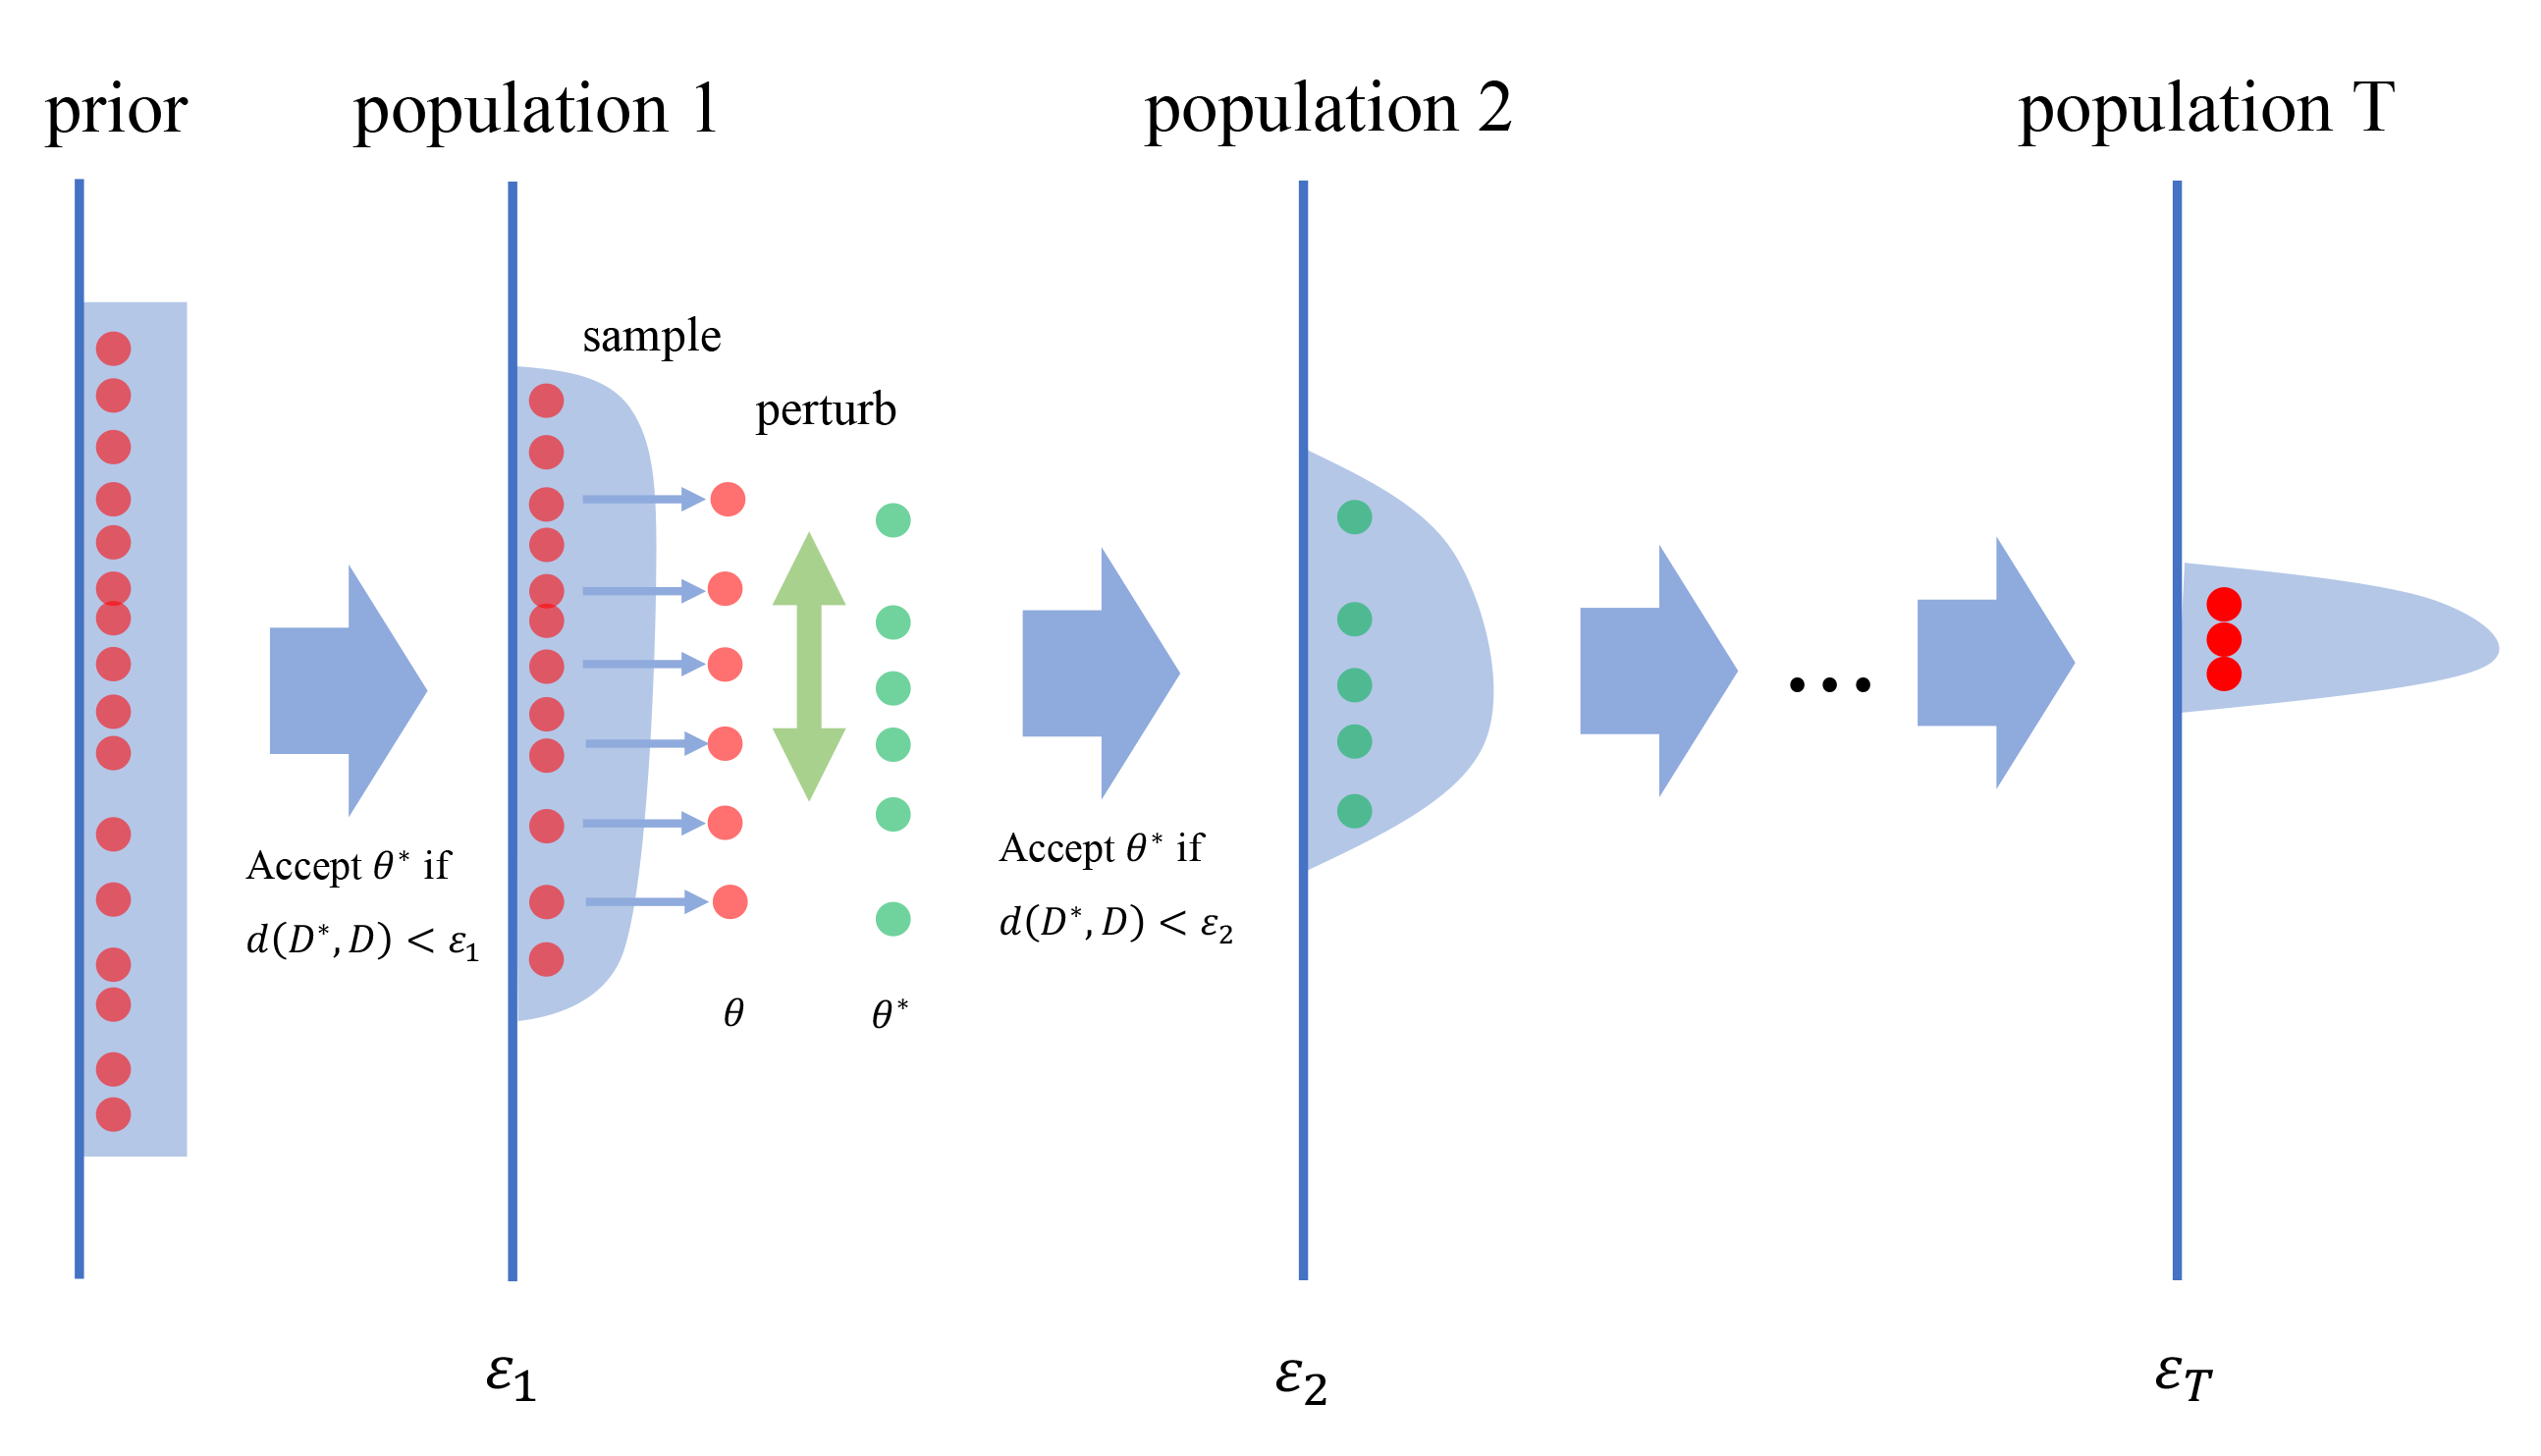
\includegraphics{fig/smc.png}}
    \end{center}

    \caption[ABC SMC sampling process]%
    {ABC SMC sampling process. $\theta^*$ denotes a sample drawn from previous population, which is used to generate simulated data $D^*$. $d$ is a distance measurement, $d(D^*,D)$ represents the discrepancy between observed data and simulated data. for each population $t$, $\epsilon_t$ is a threshold criterion to determine whether to accept that drawn sample}
    \label{fig:smc}

\end{figure}

In addition, ABC SMC is also capable of model selection tasks \cite{model_compare}. Instead of draw samples from prior of a single model, we can draw samples from multiple models $m_i$ and approximate $p(m_i, \theta|D)$, which is the joint probability distribution of model $m_i$ and its accepted particles $\theta$. In each generation the marginal distribution $p(m_i|D)$ can be calculated as the accepted ${\theta}$ is known, thus models can be ranked according to their probabilities.

The feature that ABC algorithm can perform likelihood-free inference makes it widely used in many dynamic modeling problems, especially in the area of biology \cite{ref:abcsysbio, ref:disease, ref:compare}. But ABC is not limited to these areas, as it can be generally used in inference tasks to give parameter estimates or model rankings. E.g., it has been successfully applied in cosmology studies \cite{cosmology}.



\section{Software tools}

%  [existing tools and software for this task]

%  [workflow and developing process]

 As we decided to apply ABC SMC on our regeneration models for its high-dimensional parameter estimation and comparison of different models, a code development and experiments workflow was expected to be built. The ABC SMC algorithm needs a whole set of mathematical environments (e.g. class of distributions, models and particles) and closely linked sampling and fitting algorithms (e.g. KDE fitting and Gaussian sampling), thus suitable platforms with related software packages are preferred. Regarding this, several packages in \verb|R| and \verb|Python| were studied.

 A software packages that integrally implement ABC SMC is preferred, and more options in the settings of the algorithm, more customisable features make it better. Moreover, as the ABC SMC itself is a computationally intensive task that contains massive parallel potentials, an ideal software package is expected to support as least one kind of parallel options e.g. multi-core, GPU accelerating and clusters. Otherwise, a modification or rewrite of the software package are expected to produce a reliable input-output framework for our parameter estimation and model selection experiments, where much more work would be introduced.

 Preliminarily \verb|pyABC| packages \cite{ref:pyabc} in \verb|Python| was chosen for implementations. \verb|pyABC| supports multiple types of parallelisation, e.g., multicore processing and distributed cluster, and supports resume stored runs, which made our experiments easier. It is well documented and flexible in customisations of the algorithm.

 Some other ABC SMC related packages were also examined and considered as backups, include ELFI \footnote{\url{https://elfi.readthedocs.io/en/latest/}}, ABC-SysBio \cite{ref:abcsysbio}, EasyABC\footnote{\url{https://cran.r-project.org/web/packages/EasyABC/index.html}}, GpABC \footnote{\url{https://github.com/tanhevg/GpABC.jl}}, etc. These packages may have their advantages (e.g. ABC-SysBio supports CUDA acceleration) and considered as alternative implementation methods, or can be used to compare performance difference.

 Additionally, some other softwares were also need for solving ODE, results analysis and visualisations. These software and hardware environments are listed in Appendix A.